\documentclass[../../main.tex]{subfiles}

\begin{document}
Since there is no a priori way of knowing which cells contain what mutations in real data, all accuracy benchmarking results must be taken from simulated data.
%XXX The accuracy of SCarborSNV's approximate phylogeny is first evaluated, as well as the calling accuracy with and without the phylogenetic inference stage of the algorithm.
SCarborSNV is compared against the two similar tools Monovar and Sci$\Phi$ on time, precision, recall and F1 score on simulated datasets with short (4000bp) genomes.

\subsubsection*{Time comparison}
The goal of SCarborSNV is to call SNVs efficiently from SCS data, and therefore the first important measure of success is the time taken by the program.
We generated datasets from simulated phylogenies with three cells up to 100 cells.
Next we compared the time taken for SCarborSNV to analyze these datasets, as well as its two competitors: Monovar and Sci$\Phi$.
We generated 33 datasets with three cells, but decreased the number of tests as the number of cells increased for practical time reasons.
Each tool was run on the exact same data; all the tools were run using default settings, on a single CPU core.
\begin{figure}[h] 
    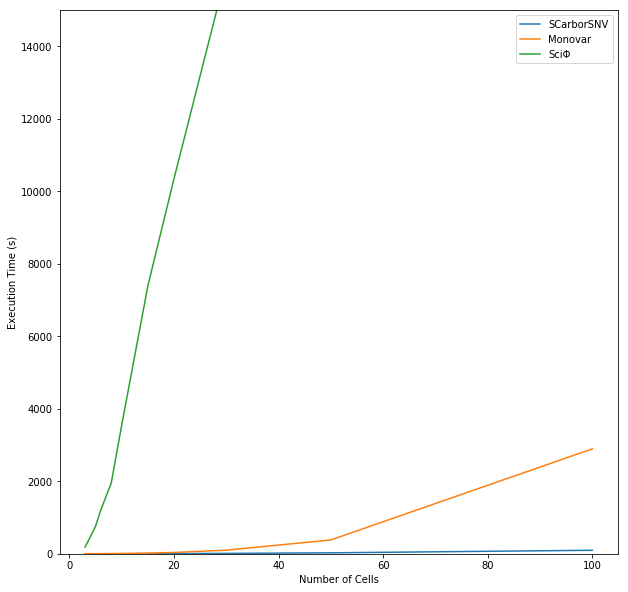
\includegraphics[width=0.9\textwidth]{sections/graphics/time}
    \caption{Average time taken by three SCS tools for 4000 simulated sites covering different numbers of related cells.
    The times are the averaged CPU times when run on an Intel\textsuperscript{\textregistered} i7-4700MQ processor running at 2.40GHz.}
    \label{fig:runningtime}
\end{figure}

As we can see in Figure~\ref{fig:runningtime}, SCarborSNV far outperformed its competition at all numbers of cells tested.
For 100 cells sequenced from a simulated genome of 4000 sites, SCarborSNV completed in just over a minute and a half while Monovar took over 48 minutes.
Even for small numbers of cells Sci$\Phi$ ran much slower than thew other two tools.
%TODO 200 cell example(?)

In these tests SCarborSNV was much faster than Monovar, which was much faster again then Sci$\Phi$.
Since SCarborSNV has an asymptotically quadratic time complexity we expect that SCarborSNV will outperform its competitors on speed by even larger margins when yet larger datasets are analyzed.

\subsubsection*{Cell calling accuracy}
As well as the time benchmarking with a variable number of cells, we benchmarked the accuracy of SCarborSNV and other tools on 100 simulated datasets with 10 cells with genomes of 4000 sites each.
We compared the results of SCarborSNV, Monovar and Sci$\Phi$ on their abilities to correctly call sites as variant, as well as calling individual cells as variant.
\begin{figure}[h] 
    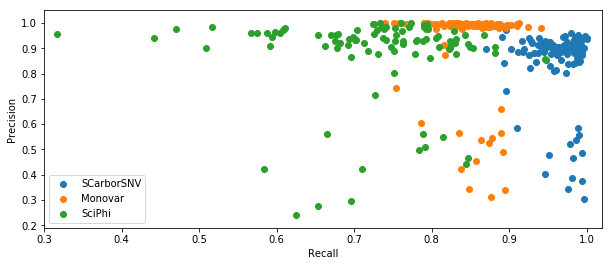
\includegraphics[width=0.9\textwidth]{sections/graphics/cell10accuracy1}
    \caption{Variant cell calling from simulated datasets of 10 cells each.}
    \label{fig:cell10accuracy1}
\end{figure}
Figure~\ref{fig:cell10accuracy1} shows that on these simulations SCarborSNV had a distinctly higher recall than Monovar, however this was at the cost of generally reduced precision.
On these datasets, Sci$\Phi$ had significantly lower recall than the other two tools, with an average precision between Monovar and SCarborSNV.
In other words SCarborSNV on average called more cells as variant, including more true variants but also more false positives.
Overall, when compared with its competitors SCarborSNV did have a better F1 score for calling cells as variant from these data, as shown in Table~\ref{table:cell10accuracy1}.
\begin{table}[h]
    \centering
    \begin{tabular}{||c|c c c||}
        \hline\hline
        Algorithm & Recall & Precision & F1 Score\\
        \hline
        SCarborSNV & 0.962 & 0.841 & 0.887\\
        Monovar & 0.849 & 0.923 & 0.873\\
        Sci$\Phi$ & 0.720 & 0.877 & 0.772 \\
        \hline\hline
    \end{tabular}
    \caption{Average recall, precision and F1 score of variant cell calling for three different algorithms benchmarked on 100 simulated datasets of 10 cells each.}
    \label{table:cell10accuracy1}
\end{table}

%TODO by number of cells

\subsubsection*{Site calling accuracy}
As well as their abilities to call individual cells as variant at different loci, we also compared the three algorithms on their ability to call one or more cells as variant at a variant locus.
In some applications it may be important to know whether certain mutations occur at all in any subpopulation of cells, so this is also an important metric.

\begin{figure}[h] 
    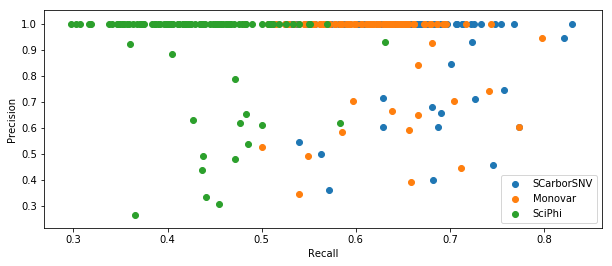
\includegraphics[width=0.9\textwidth]{sections/graphics/site10accuracy1}
    \caption{Variant site calling from simulated datasets of 10 cells each.}
    \label{fig:site10accuracy1}
\end{figure}

Figure~\ref{fig:site10accuracy1} shows the precision and recall of calling sites as variant for the three algorithms SCarborSNV, Monovar and Sci$\Phi$.
In this measurement, SCarborSNV on average had better precision, recall and F1 score than Monovar, as shown in Table~\ref{table:site10accuracy1}.
Sci$\Phi$ performed poorly on these simulations, with similar precision to the other tools but on average significantly lower recall.

\begin{table}[h]
    \centering
    \begin{tabular}{||c|c c c||}
        \hline\hline
        Algorithm & Recall & Precision & F1 Score\\
        \hline
        SCarborSNV & 0.652 & 0.943 & 0.763\\
        Monovar & 0.617 & 0.941 & 0.737\\
        Sci$\Phi$ & 0.431 & 0.935 & 0.579 \\
        \hline\hline
    \end{tabular}
    \caption{Average values for site calling for three different algorithms for the 100 simulated datasets of 10 cells each.
    Generally the accuracy for site calling is lower than that for cell calling since there are many sites with only one or two mutant cells each, and these sites are challenging to call accurately.}
    \label{table:site10accuracy1} 
\end{table}

\subsubsection*{Tree accuracy}
A common way to compare unrooted labeled phylogenies is using the Robinson-Foulds metric.
This distance measure between two phylogenies is based on the fact that a phylogenetic tree implies certain partitions of the set of terminal clades.
The RF metric is equal to the sum of both the number of partitions implied by tree 1 that are not implied by tree 2, as well as the number of partitions implied by tree 2 that are not implied by tree 1~\cite{RFmetric}.

There is a similar value that can be computed for rooted trees that is based on clusters rather than partitions.
This rooted Robinson-Foulds metric can be normalized empirically by comparing the metric to the average distance between randomly generated trees.
In this way a normalized metric of 0 implies the exact same phylogeny, and a metric of 1 implies that the two phylogenies are only as similar as two random trees on average.
We use the tool TreeCmp to compute this metric between the simulated tree and inferred tree for both the trees created my SCarborSNV and Sci$\Phi$.
TreeCmp has empirically calculated the normalization values for trees with different numbers of leaves beforehand~\cite{TreeCmp}.

On the 100 10-cell datasets, Sci$\Phi$ recovered trees more accurately than SCarborSNV, with an average normalized rooted Robinson-Foulds metric of 0.752 compared with 0.798 for SCarborSNV.
The normalized Robinson-Foulds metric for these 100 datasets is summarized in Figure~\ref{fig:RFviol}.

\begin{figure}[h] 
    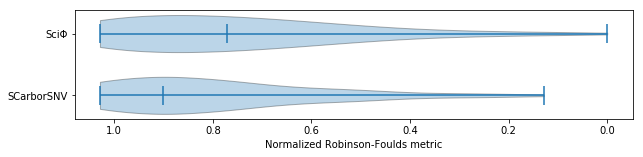
\includegraphics[width=0.9\textwidth]{sections/graphics/RFviolinplots}
    \caption{Violin plots of the normalized Robinson-Foulds metric between the ground truth phylogenies and those inferred by each tool.
    A lower value of the RF metric indicates more accurate recovery of the simulated phylogeny.}
    \label{fig:RFviol}
\end{figure}

\subsubsection*{Phylogenetic inference}
Plot of precision vs recall for initial call and phylo call. Hopefully phylo call increases.

\end{document}

